..\chapter{System}
In this chapter, we discuss about the system overview for traffic light detection.
This system detect the color of traffic light in a recorded videoframe.
We captured video using a smartphone along with the sensor data.

\section{System architecture}
\label{s:archi}
We use three features of traffic light, color,shape, and traffic bulb in a black box and the sensor feature of a smartphone as a system architecture for traffic light detection.
While recording the video we logged in the sensor data.
The first step of detection is the color filtering of the recorded videos.
Each video frames is consist of different colors.
In this step each frame is filtered with only red and green pixel.
The traffic bulb shape is mostly circle.
To detect this characteristic we use Hough Circle  transformation\cite{hough_circle}.
Based on the traffic light detection position in videoframes, we fix region of interest area, which is a subpart of videoframes.
After that, on next videoframes the ROI change in respect to the sensor data. 

\subsection{Diagram}

Section \ref{s:archi} discesses the overall architecture of our system.

\ref{f:sys_dia} shows the overview of the system.

\begin{figure}
\centering
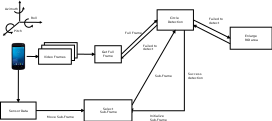
\includegraphics[width=5.2in]{figures/sysdia.png}
\caption{System Overview}
\label{f:sys_dia}
\end{figure}

At first we recorded videos along with the sensor data, gyroscope, accelerometer, pitch,roll, and azimuth.
These data have syncronization with our recorded videoframes, since we logged in sensor data while recording.
Now to detect the traffic light, we use three features of traffic light.
Those are the color, shape of traffic light and traffic light location in a black box.
For detection using the color and shape features,we need to filter out the frames with the red and green pixel value.
For this purpose we convert the BGR color space to HSV space first.
In BGR space, to detect specific color we need to depend on three different values (B,G,R)
HSV space has the property to find out the color based on only single value,hue.
The range of hue values of each color are well defined that help us to filter out our desired pixels.
In OpenCV the hue range is from 0 to 180.
We fix the range for red and green analysing the color range of traffic bulbs.
\ref{t:hue_range} shows the hue range for red and green pixel.

\begin{table}[h!]
  \centering
  \caption{Hue range for red and green pixel.}
  \label{t:hue_range}
  \begin{tabular}{  l | c  }
    \hline
    Hue range for red & Lower 0 to 10 \\ \cline{2-2}
    & Upper 160 to 179 \\
    \hline \hline
    Hue range for green & 65 to 95 \\
    \hline
  \end{tabular}
\end{table}

Before use these filter images to detect circle, we use gaussian blur filter, in order to avoid false detection.
After this, we use the circle Hough Transform \cite{hough_circle} to detect the circles.
But, noise from the original images can fool the hough transform to detect false and more circles.
As a solution to this poblem, before converting our original BGR space frame to HSV space, a median filter is used.
Now to detect if traffic light is in the black box, the other feature of our detection, we scan a rectangle frame  around the traffic light.
Traffic lights locate in a black box, which can place in horizontally or vertically in street.
To make our approch more global we scan all around the traffic light to check the intensity.
The intensity of black color can detect to check the Value of HSV space.
For black color, range of Value is very low, less than 40-45.
\ref{f:norec_filter} shows there is one green false positive between two red traffic light.
\ref{f:rec_filter} shows the output after using our heuristic black box checking filter.


\begin{figure}
\centering
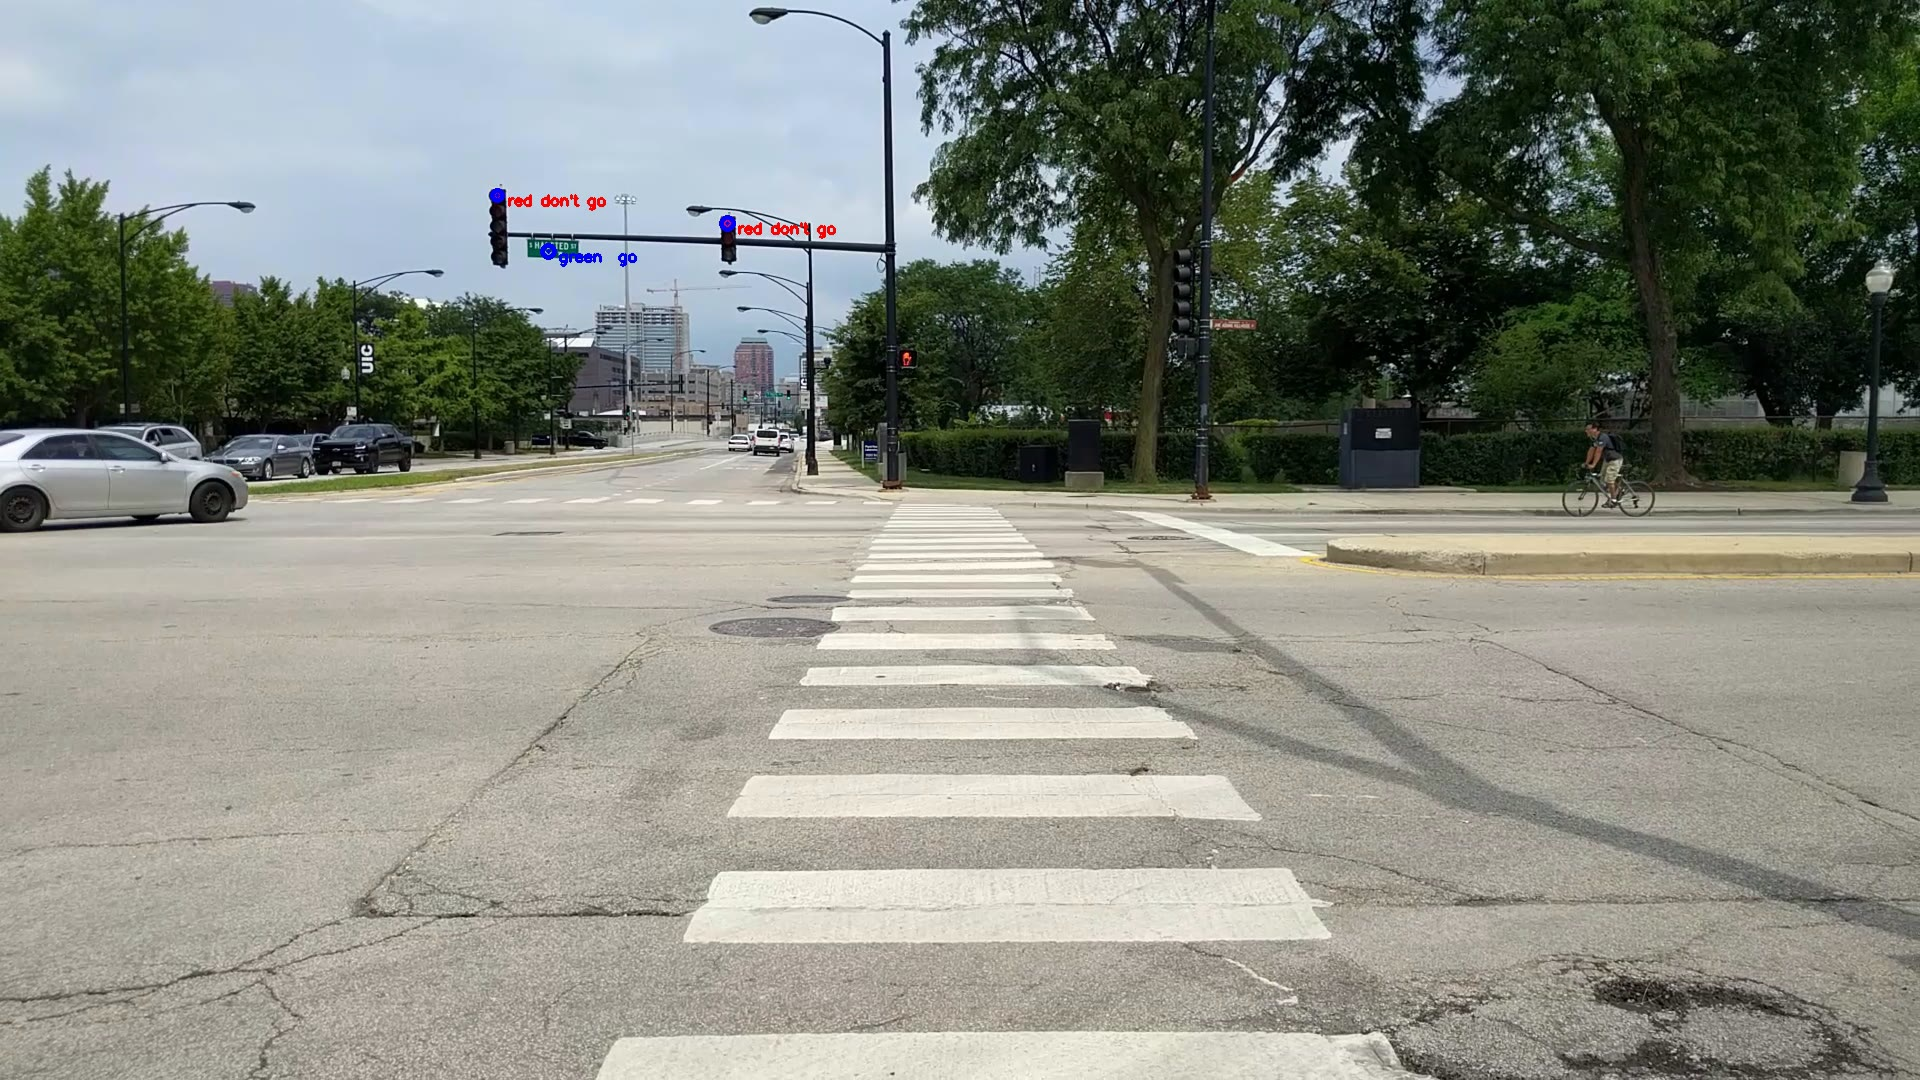
\includegraphics[width=5.2in]{plots/norec_filter.jpg}
\caption{Output not using black box checking filter.}
\label{f:norec_filter}
\end{figure}

\begin{figure}
\centering
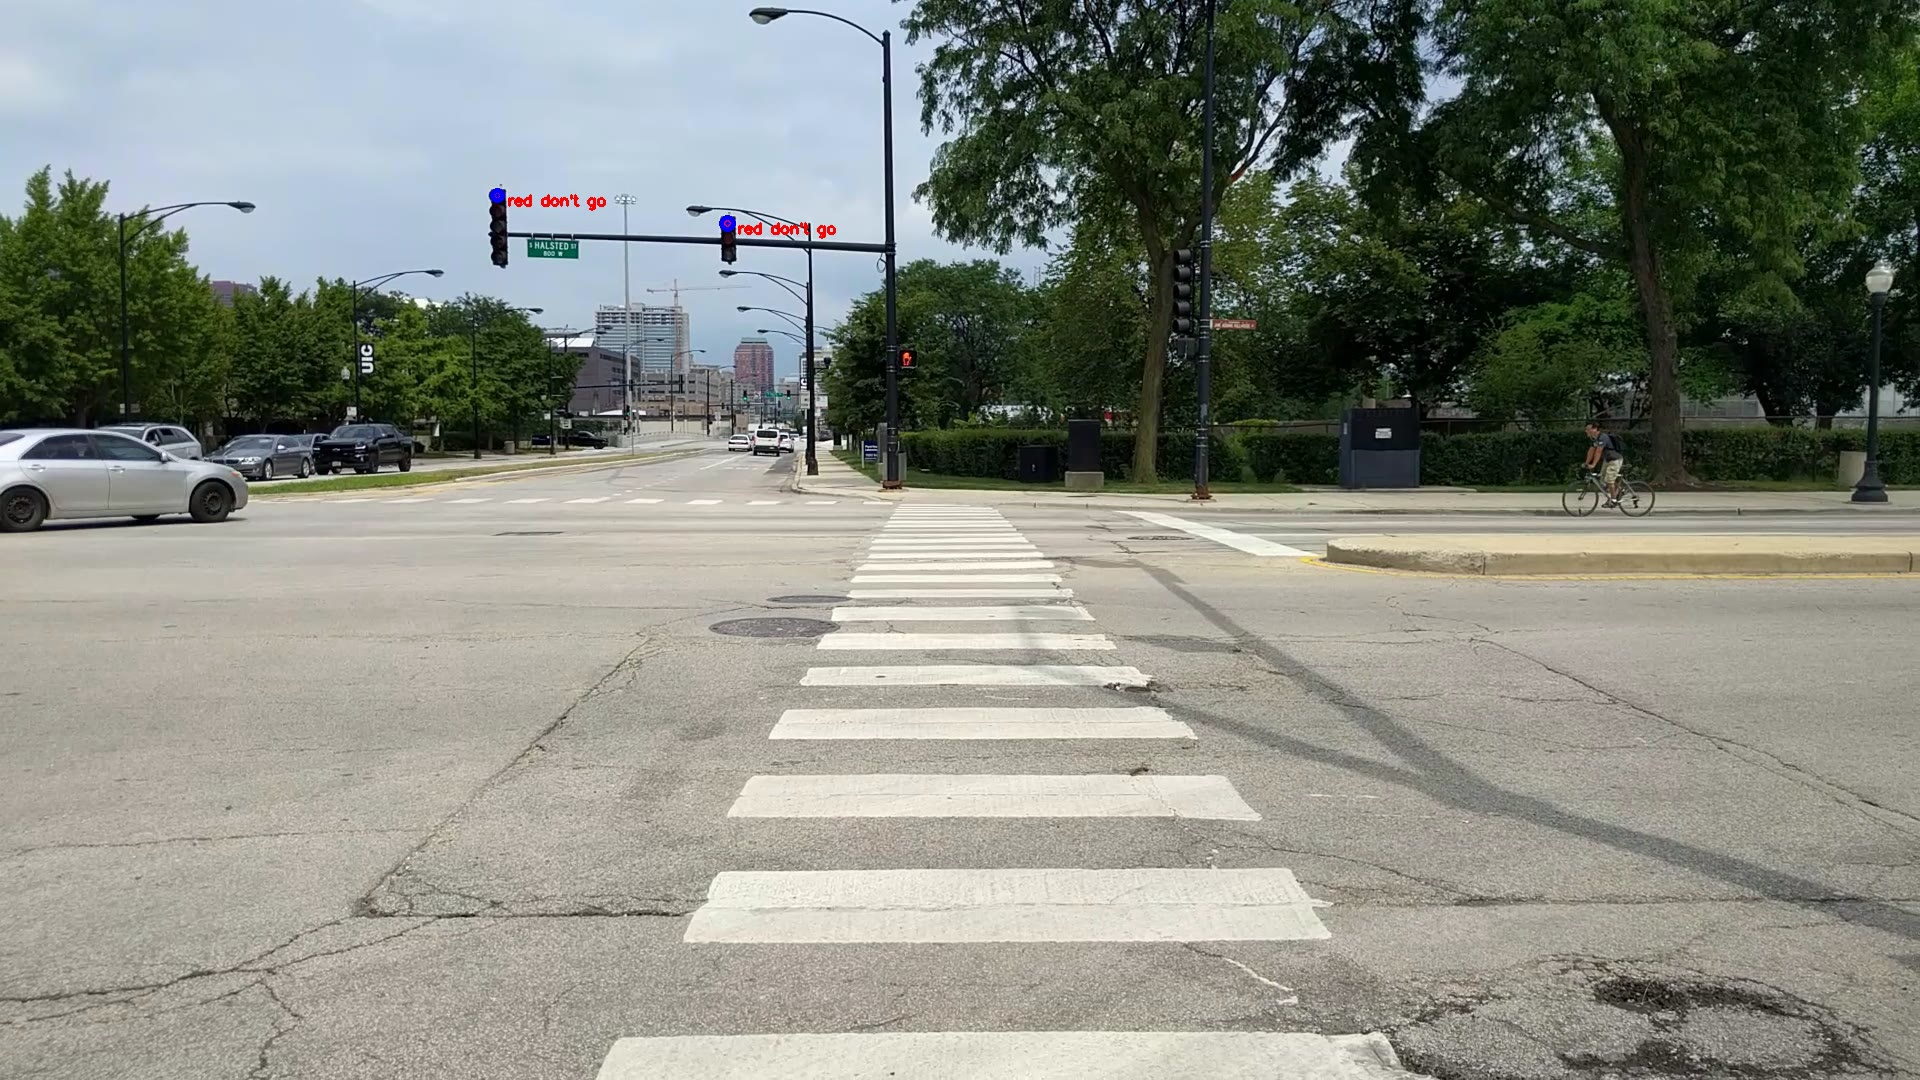
\includegraphics[width=5.2in]{plots/rec_filter.jpg}
\caption{Output using black box checking filter.}
\label{f:rec_filter}
\end{figure}

For improvize our detection we also use the smartphone sensor data.
So when we detect a traffic light in our video frame successfully using the color,shape of traffic light and the characteristics of traffic bilb being in a box, we have idea of the position of the traffic light.
With this idea we subdevide our videoframe making a region of interest area.
When we move to the next frame, we have a prior knowledge of traffic light position and we know the sensor data, pitch, roll and azimuth of this frame.
Using these sensor data of curent frame and the previous frame we have the idea of movement of traffic light.
With this change of movement the ROI also moves to the direction of change.
\ref{f:rec_mv}shows the movement of ROI with the change of pitch and azimuth of our recorded video.
Apart from this, when our system can not detect any circle in our specific ROI area, it updates the ROI and try to detect the light.

\begin{figure*}[!ht]
\centering
\subfloat[Initial ROI] {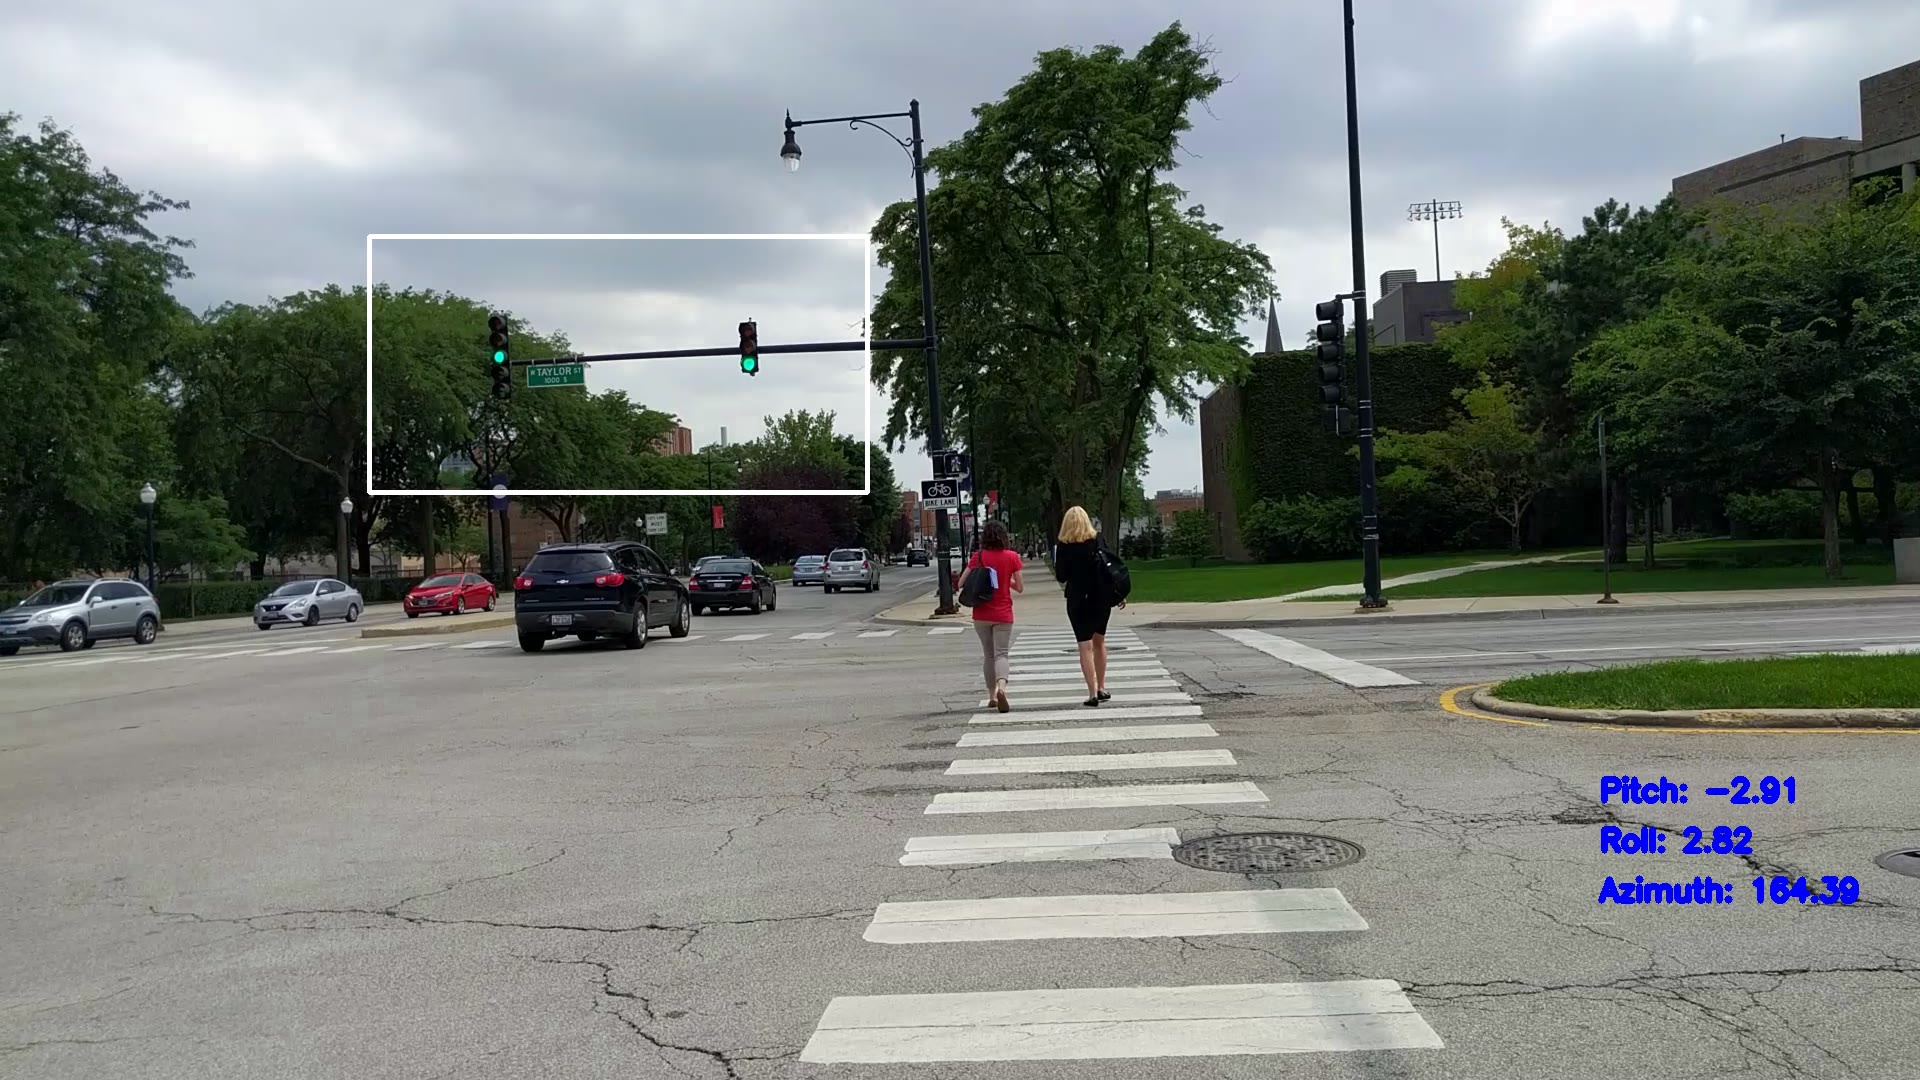
\includegraphics[width=3.2in]{plots/rec_mv.jpg}}
\subfloat[Movement with change of sensor data] {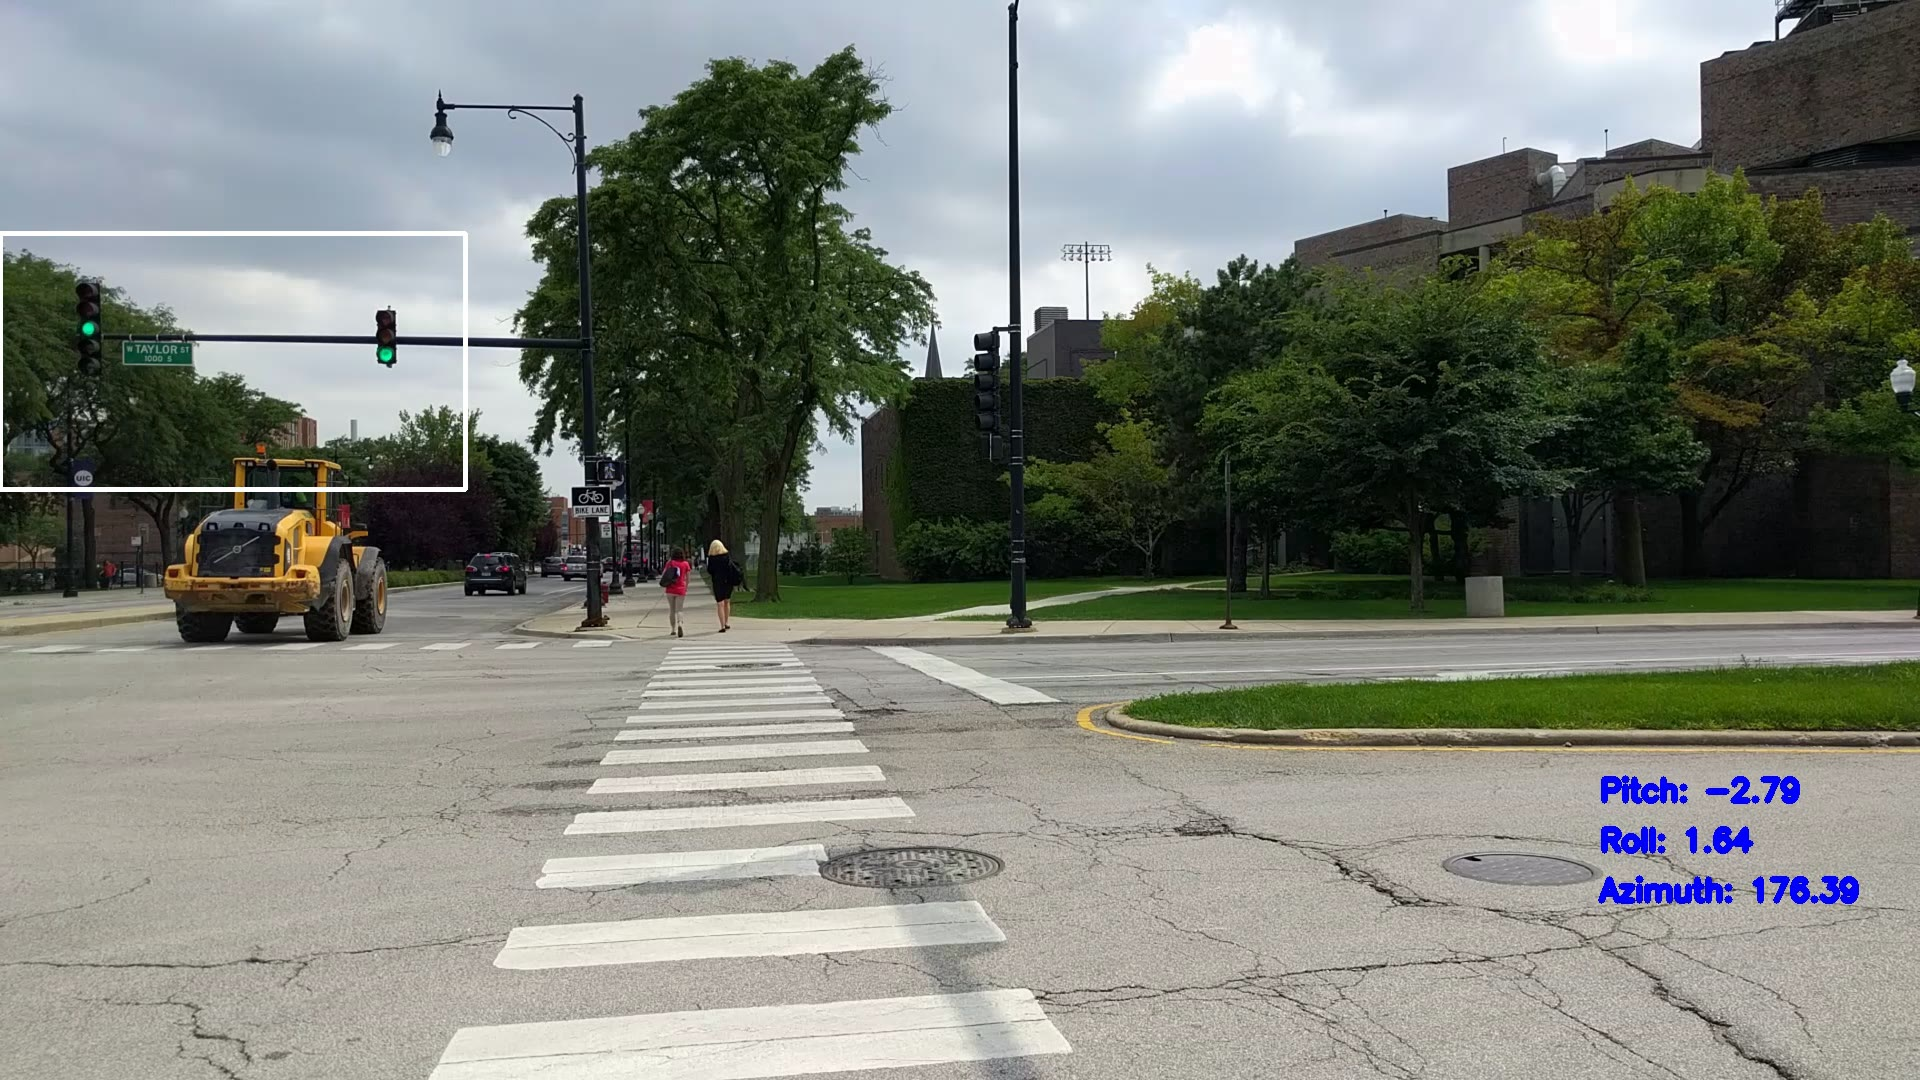
\includegraphics[width=3.2in]{plots/rec_mv1.jpg}}\\
\subfloat[Movement] {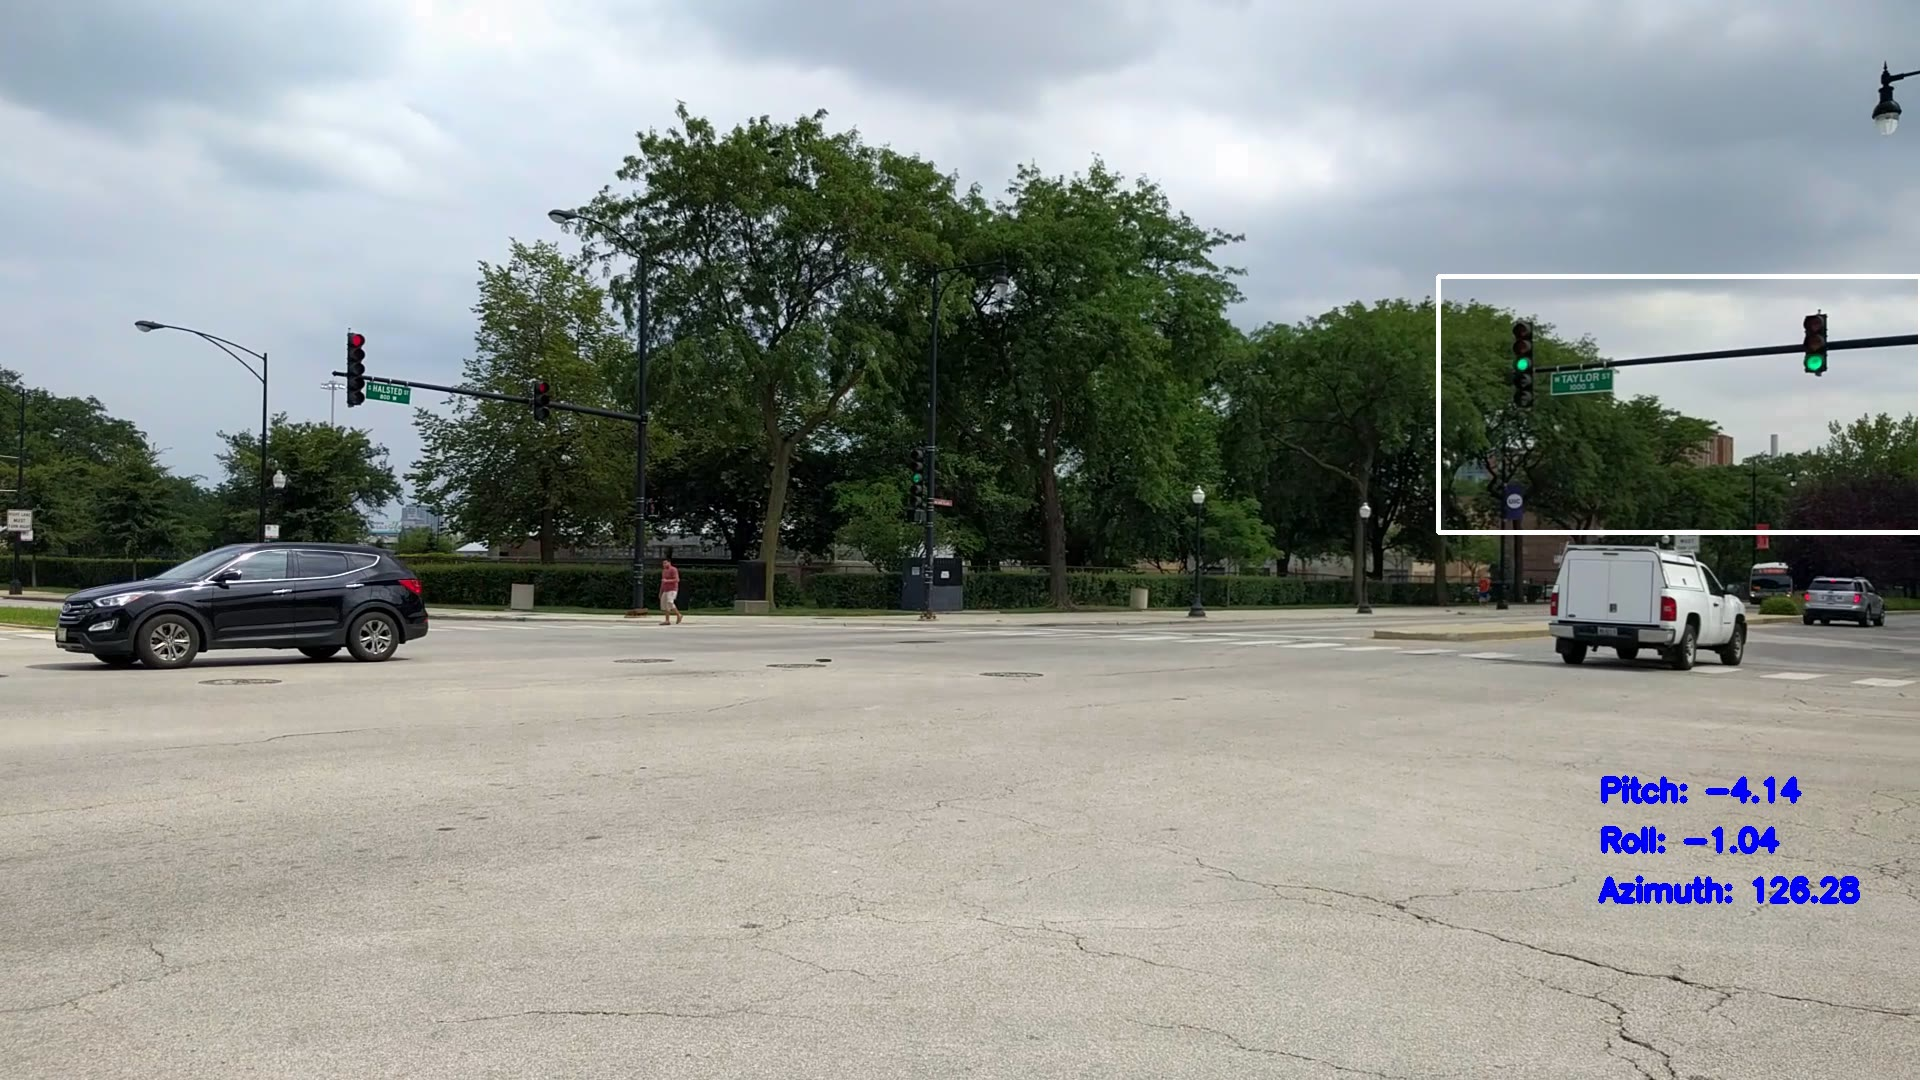
\includegraphics[width=3.2in]{plots/rec_mv2.jpg}}

\caption{ROI movement with the change of sensor data.}
\label{f:rec_mv}
\end{figure*}


With the successful detection, our region of interest again change with the light position and pitch and azimuth value.
For unsuccessful detection, ROI enlarged until it process the full frame and then go to the next frame to detect traffic light.
And this process is contuing to every frame.

\begin{figure*}[!ht]
\centering
\subfloat {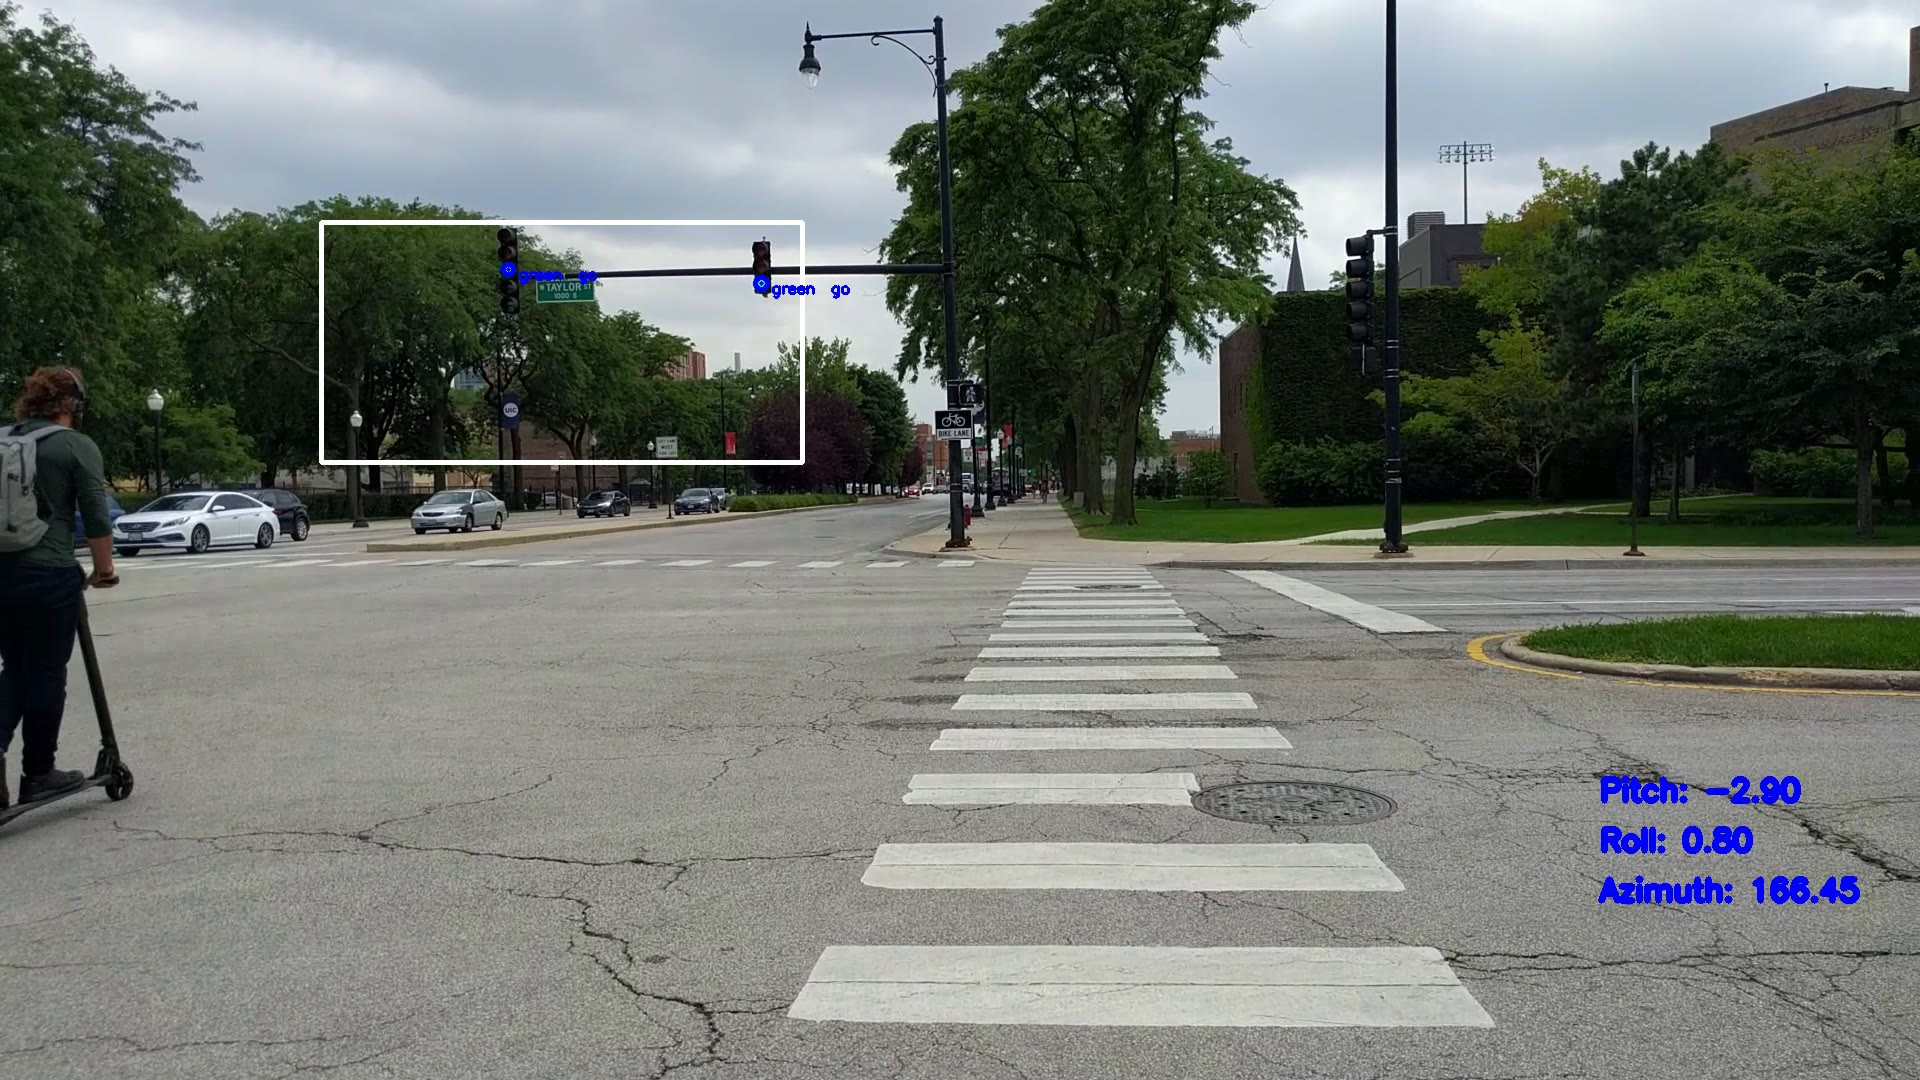
\includegraphics[width=3.2in]{plots/rec_enl.jpg}}
\subfloat {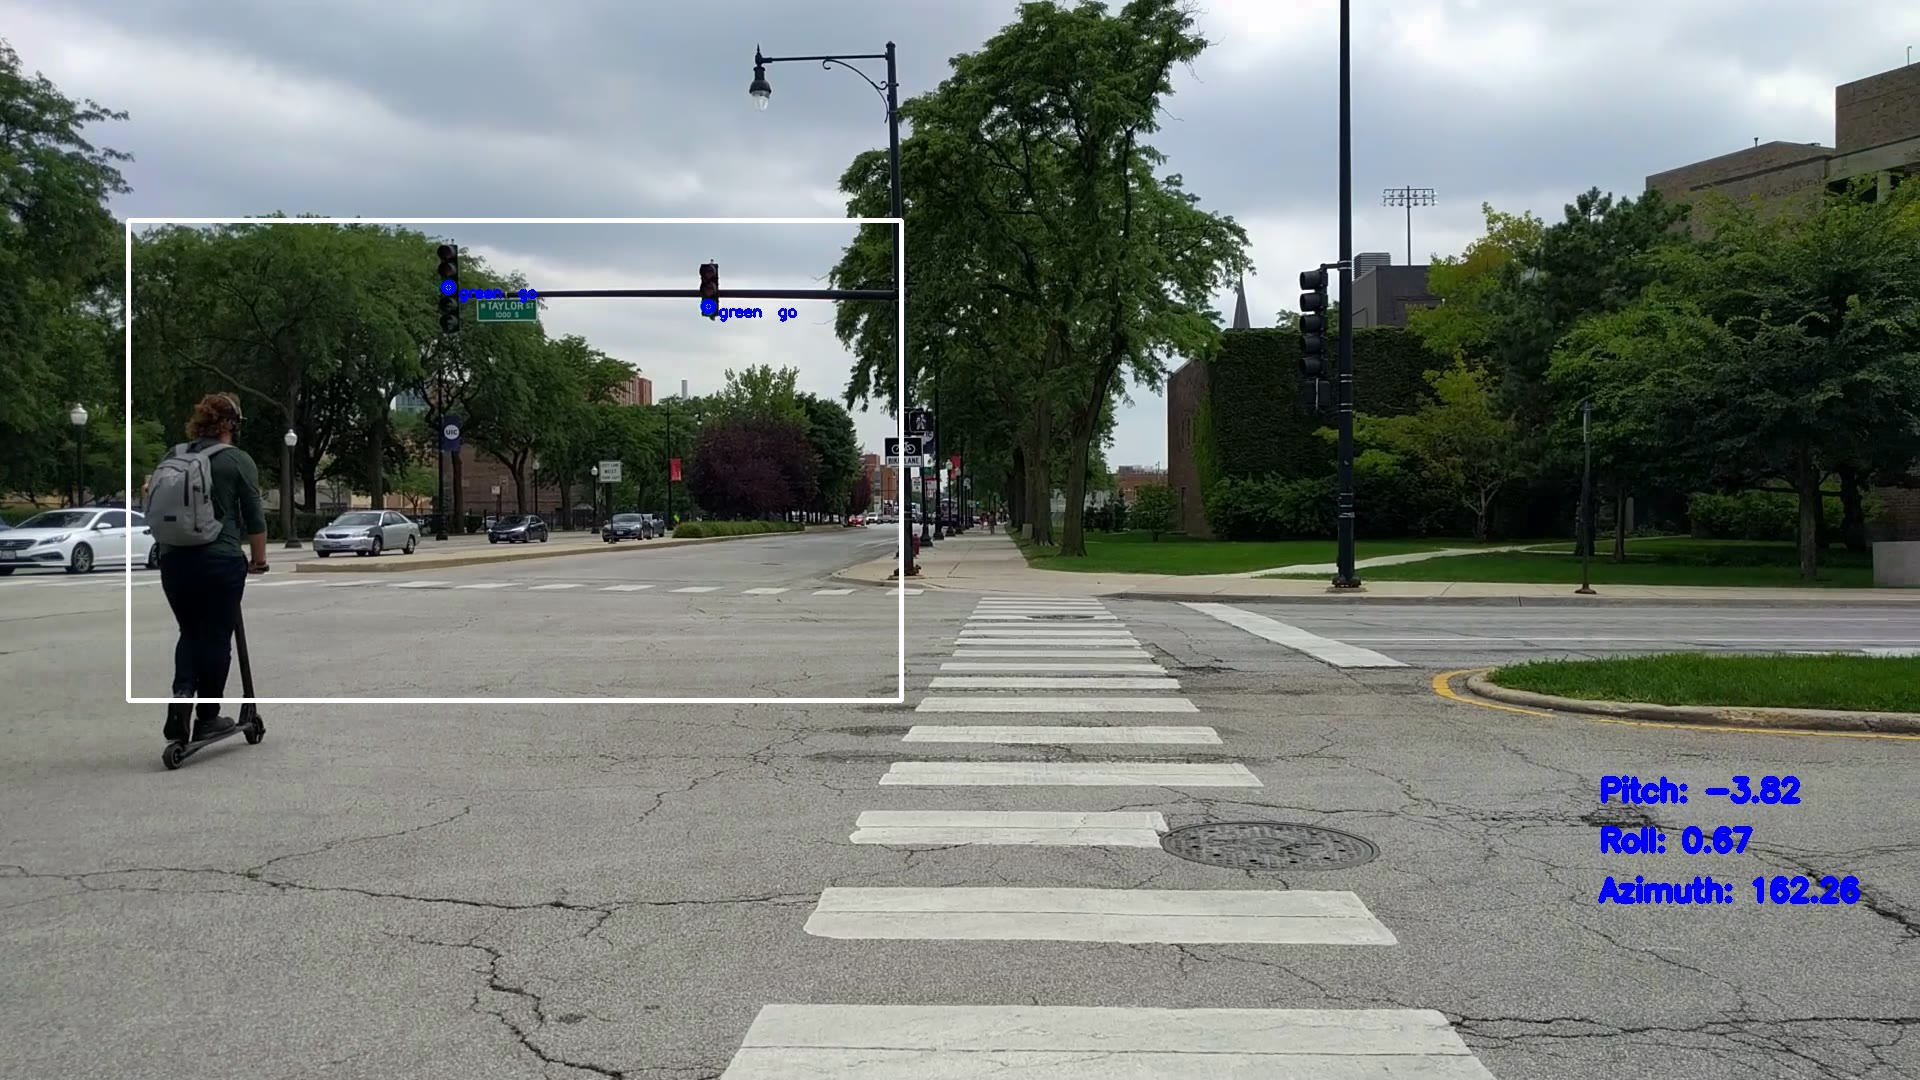
\includegraphics[width=3.2in]{plots/rec_enl1.jpg}}

\caption{Enlarged ROI to detect traffic light successfully.}
\label{f:rec_enl}
\end{figure*}




\begin{figure}
\centering
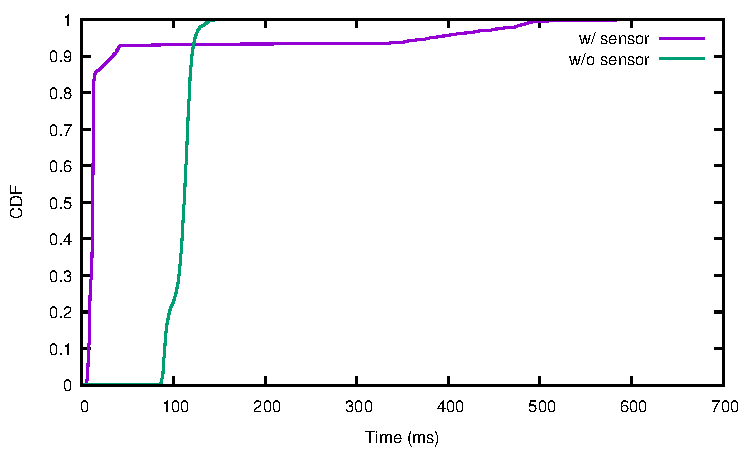
\includegraphics[width=5.2in]{plots/cdf_time.pdf}
\caption{CDF of frame processing time.}
\label{f:cdf_time}
\end{figure}


